\subsubsection{Integrity check}
\label{sec:sphinx:integrity}

Upon reception of a packet, each node first derives the shared key $s_i$ with the creator of the packet. Before it unblinds the routing information, it checks their integrity and \textit{should} drop the packet if the header has been tampered.

\paragraph{Integrity tag}

As by section \ref{sec:sphinx:keyderivation}, each node along the path shares a secret $s_i$ with the creator of the packet. To create an integrity tag $\gamma_i$, the node first derives a sub-key $s_i^{int}$ as described in appendix \ref{appendix:keyderivation}, yielding:

$$\gamma_i = HMAC_{s_i^{int}}(\beta_i)$$

where $HMAC$ is instantiated with the hash function \textsf{BLAKE2s} and the output size is set to 32 bytes.

\paragraph{Packet transformation} tbd

\begin{figure}[H]
    \centering
    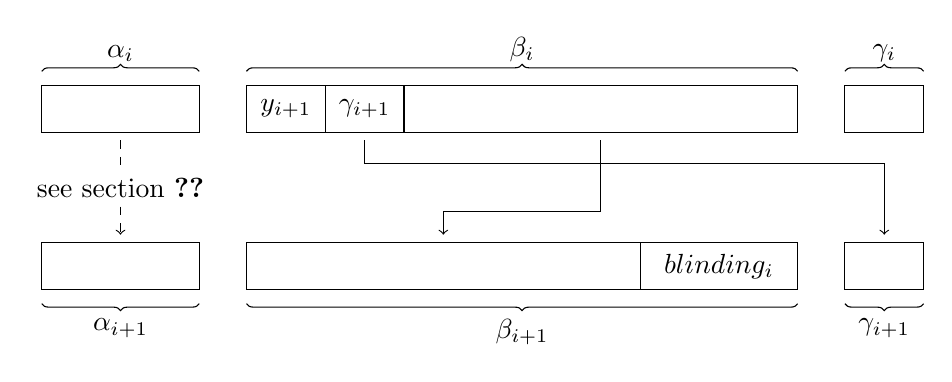
\begin{tikzpicture}
        \def\one{0.6}
        \def\alphaLength{2.0}
        \def\betaLength{7.0}
        \def\betaOffset{1.0}
        \def\gammaLength{1.0}
        \def\padding{0.6}
        \def\secondPacket{-2}

        \foreach \offset\i in{0/0,\secondPacket/1} {
                \begin{scope}[shift={(0,\offset)}]
                    \ifnum\i=0
                        \draw[decoration={brace,raise=5pt},decorate] (0,\one) -- node[above=5pt] {$\alpha_{i}$} (\alphaLength,\one);
                        \draw[->,dashed] (\alphaLength*0.5,-0.1) -- (\alphaLength*0.5,\secondPacket+\one+0.1) node [midway,fill=white] {see section \ref{sec:sphinx:keyderivation}};
                    \else
                        \draw[decoration={brace,raise=5pt,mirror},decorate] (0,0) -- node[below=7pt] {$\alpha_{i+1}$} (\alphaLength,0);
                    \fi
                    \draw (0,0) rectangle (\alphaLength,\one);

                    \begin{scope}[shift={(\alphaLength+\padding,0)}]
                        \ifnum\i=0
                            \draw[decoration={brace,raise=5pt},decorate] (0,\one) -- node[above=5pt] {$\beta_{i}$} (\betaLength,\one);
                            \draw (0,0) rectangle (\betaOffset,\one) node [midway] {$y_{i+1}$};
                            \draw (\betaOffset,0) rectangle (\betaOffset+\betaOffset,\one) node [midway] {$\gamma_{i+1}$};

                            \draw[->] (\betaOffset+\betaOffset*0.5,-0.1) -- (\betaOffset+\betaOffset*0.5,-0.4) -- (\padding+\betaLength+\gammaLength*0.5,\secondPacket+\one+0.1+0.9) -- (\padding+\betaLength+\gammaLength*0.5,\secondPacket+\one+0.1);

                            \draw[->] (\betaOffset+\betaLength*0.5,-0.1) -- (\betaOffset+\betaLength*0.5,-0.1-0.9) -- (\betaLength*0.5-\betaOffset,-0.1-0.9) -- (\betaLength*0.5-\betaOffset,\secondPacket+\one+0.1);
                        \else
                            \draw[decoration={brace,raise=5pt,mirror},decorate] (0,0) -- node[below=7pt] {$\beta_{i+1}$} (\betaLength,0);
                            \draw (\betaLength-\betaOffset-\betaOffset,0) rectangle (\betaLength,\one) node [midway] {$blinding_i$};
                            \draw (\betaLength-2*\betaOffset,0) -- (\betaLength-2*\betaOffset,\one);
                        \fi


                        \draw (0,0) rectangle (\betaLength,\one);
                    \end{scope}

                    \begin{scope}[shift={(\alphaLength+\padding+\betaLength+\padding,0)}]
                        \ifnum\i=0
                            \draw[decoration={brace,raise=5pt},decorate] (0,\one) -- node[above=5pt] {$\gamma_{i}$} (\gammaLength,\one);
                        \else
                            \draw[decoration={brace,raise=5pt,mirror},decorate] (0,0) -- node[below=7pt] {$\gamma_{i+1}$} (\gammaLength,0);
                        \fi
                        \draw (0,0) rectangle (\gammaLength,\one);
                    \end{scope}
                \end{scope}
            }

    \end{tikzpicture}
    \caption{Extraction of $\gamma_{i+1}$ and creat}
\end{figure}

\paragraph{Filler}

In order to compute the integrity tag, the sender needs to know \textit{how} the packet is going to look like once it reaches the node that checks its integrity. Hence, the creator of the packet needs to perform the whole transformations that are done by the relayers along the path \textit{in advance} before sending the packet.

\begin{figure}[H]
    \centering
    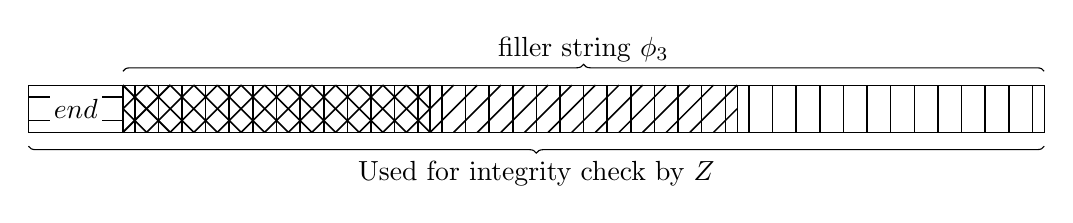
\begin{tikzpicture}
        \def\one{0.6}
        \def\scale{0.9}
        \def\nodeWidth{1.95}
        \def\endWidth{1.2}
        \def\width{3*2*\nodeWidth+\endWidth}
        \foreach \i\name in{0/B,1/C,2/D,3/Z} {
                \ifnum\i=3
                    \def\a{11.7}
                    \def\diff{11.1}
                \fi

                \ifnum\i=2
                    \def\a{7.8}
                    \def\diff{7.2}
                \fi

                \ifnum\i=1
                    \def\a{3.9}
                    \def\diff{3.3}

                \fi

                \ifnum\i=0
                    \def\a{\endWidth}
                    \def\diff{0.6}
                \fi


                \def\b{0.6}
                \def\lw{0.2}

                \begin{scope}[shift={(\endWidth,0)}]
                    \ifnum\i=1
                        \foreach \x [count=\i] in{0,0.3,0.6,...,\b}{
                                \draw [line width=\lw mm](\x,0)--(0,\x) (\a-\b+\x,\b)--(\a,\x);
                            }
                        \foreach \x [count=\i] in{0,0.3,0.6,...,\diff}{
                                \draw [line width=\lw mm](\x+\b,0)--(\x,\b);
                            }
                    \fi

                    \ifnum\i=2
                        \foreach \x [count=\i] in{0,0.3,0.6,...,\b}{
                                \draw [line width=\lw mm](0,\x)--(\b-\x,\b) (\a-\b+\x,0)--(\a,\b-\x);
                            }
                        \foreach \x [count=\i] in{0,0.3,0.6,...,\diff}{
                                \draw [line width=\lw mm](\x,0)--(\b+\x,\b);
                            }
                    \fi

                    \ifnum\i=3
                        \foreach \x [count=\i] in{0.15,0.45,...,\a}{
                                \draw [line width=\lw mm](\x,0)--(\x,\b);
                            }
                    \fi
                \end{scope}

                \ifnum\i=0
                    \foreach \x [count=\i] in{0.15,0.45,...,\b}{
                            \draw [line width=\lw mm](0,\x)--(\a,\x);
                        }
                \fi
                \ifnum\i>0
                    \draw (\i*2*\nodeWidth+\endWidth,0) -- (\i*2*\nodeWidth+\endWidth,\one);
                \else
                    \draw [color=white] (\i*2*\nodeWidth,0) rectangle (\i*2*\nodeWidth+\endWidth,\one) node [midway,color=black,fill=white,inner sep=1.5pt] {$end$};
                    \draw (\endWidth,0) -- (\endWidth,\one);
                \fi
            }

        \draw (0,0) rectangle (\width,\one);
        \draw[decoration={brace,raise=5pt},decorate] (\endWidth,\one) -- node[above=5pt] {filler string $\phi_3$} (\width,\one);
        \draw[decoration={brace,mirror,raise=5pt},decorate] (0,0) -- node[below=7pt] {Used for integrity check by $Z$} (\width,0);

    \end{tikzpicture}
    \caption{Transformed header as seen by $Z$}
\end{figure}

Since each node, shifts the routing information to left, thereby deletes their own routing information and appends their own padding in the end, the routing information of the very last node consists of the $END$ message as desribed section \ref{sec:sphinx:routinginformation} and the padding that got appended by the previous nodes. To compute the integrity tag for that node, the creator of the packet needs to compute a filler string $\phi$ and use it to compute

$$\gamma_i = HMAC_{s_i^{int}}(END \ || \ \phi_i )$$
